\documentclass[addpoints, 12pt] {exam}
\usepackage{graphicx}
\usepackage{amsmath}
\bracketedpoints
\pagestyle{headandfoot}
\runningheadrule
\firstpageheader{Math 112}{Written Homework 6}{Due February 23rd 2023}
\runningheader{Math 112}{ Page\; \thepage\; of\; \numpages}{Written Homework 6}
\firstpagefooter{}{}{}
\runningfooter{}{}{}
\setlength\answerskip{2ex}
\setlength\answerlinelength{1.5in}
\begin{document}

\begin{center}
\fbox{\fbox{\parbox{5.5in}{\centering
Directions:\\Please only put your final, well written solutions, in the space provided.\\ Give exact answers (simplified radicals or fractions).\\If you use additional paper clearly label the question and upload pages after the question page.\\Use complete sentences and explain your reason as much as possible.\\There are \numquestions\,  questions and \numpoints\, points total
}}}\end{center}
\vspace{0.1in}
\makebox[\textwidth]{Name:\enspace\hrulefill}
%\qformat{Question \thequestion \dotfill \thepoints}%

\begin{questions}
\question \begin{parts}\part[2] Suppose that we are considering two functions, \(f(x)\) and \(T(x)\). Provide the definition (and state the correct name) for the expression:\((f\circ T)(x)\)\vspace{0.5in}
\part Let \(f(x) = x^2-3\) and \(T(x) = \sqrt{x+12} \). Show all work and answer each question below.
\begin{subparts}
\subpart[1] Evaluate \((f\circ T)(4)\).  \vspace{0.5in} \answerline
\subpart[1] Evaluate \((T\circ f)(4)\). \vspace{0.5in}\answerline
\subpart[2] What is \((f\circ T)(x)\)?\vspace{0.5in}\answerline
\subpart[2] What is \((T\circ f)(x)\)?\vspace{0.5in}\answerline
\subpart[2] 
\end{subparts}\end{parts}\newpage

\question For each part below, consider the functions \(f(x)=x^2-16\), \(g(x) = \displaystyle\frac{1}{x-4}\), and \(h(x) =\displaystyle\frac{1}{x}\).
\begin{parts}
\part[3] Evaluate and simplify \(A(x)=\left(\frac{f}{g}\right)(x)\).\vspace{1in}\answerline

\part[2]Evaluate and simplify \(B(x)=(g+h)(x)\)\vspace{1in}\answerline

\part[2]Evaluate and simplify \(C(x)=(g\circ h)(x)\)\vspace{1in}\answerline
\part For each of the new functions, \(A(x)\), \(B(x)\), and \(C(x)\), what is the domain of each function?
\begin{subparts}
\subpart[1] Domain of \(A(x)\):\answerline
\subpart[1] Domain of \(B(x)\):\answerline
\subpart[1] Domain of \(C(x)\):\answerline
\end{subparts}
\end{parts}\newpage

\question Use the graph of \(R(x)\) and \(G(x)\) below to answer the questions. Please use \emph{interval} notation where appropriate.\begin{center}
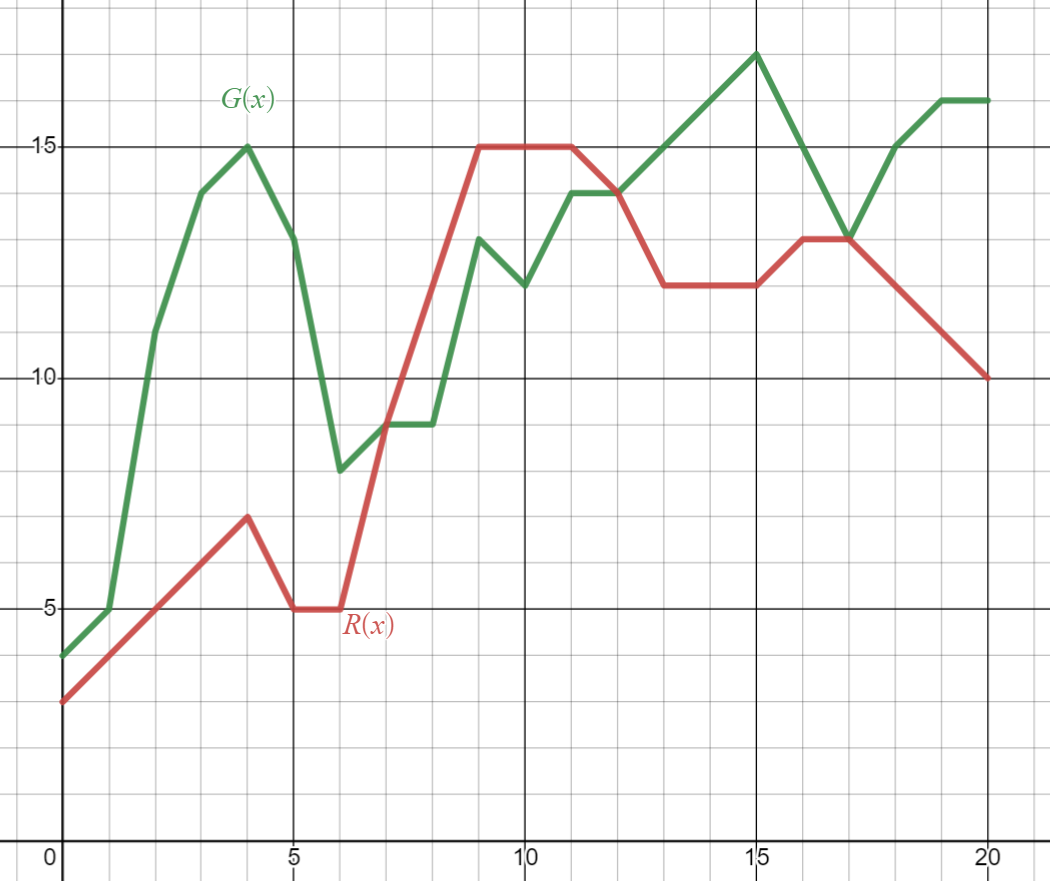
\includegraphics[scale=0.4]{RandG}\end{center}
 \begin{parts}
 \part[1]What is the range of \(G(x)\)?\answerline
 \part[1]What is the range of \(R(x)\)?\answerline
 \part[1]Where is \(R(x)\) increasing?\answerline
 \part[1]Where is \(G(x)\) constant?\answerline
 \part[2]Where is \((R-G)(x)\) positive?\answerline
 \part[2]Where is \((R-G)(x)\) negative?\answerline
 \part[2]Where is \((R-G)(x)\) zero?\answerline
 \end{parts}\newpage
\question The following table records the number of motor vehicle crash deaths for teens between the age of 13-19, separated by gender for the years 2005-2015 (Data source: iihs.org)
$$
\begin{array}{|c|c|c|c|c|}\hline
\textbf{Year }t&\textbf{Male }M(t)&\textbf{Female }F(t)&(M+F)(t)&(M-F)(t)\\\hline
2005&3,496&1,803&&\\\hline
2006&3,415&1,744&&\\\hline
2007&3,280&1,701&&\\\hline
2008&2,694&1,373&&\\\hline
2009&2,222&1,257&&\\\hline
2010&2,034&1,087&&\\\hline
2011&1,991&1,041&&\\\hline
2012&1,863&972&&\\\hline
2013&1,661&880&&\\\hline
2014&1,802&828&&\\\hline
2015&1,788&926&&\\\hline
\end{array}$$
\begin{parts}
\part[2]Fill in the missing columns, \((M+F)(t)\) and \((M-F)(t)\).
\part[1]Provide a practical description for what the \((M+F)(t)\) column means.\vspace{1in}
\part[1]Provide a practical description for what the \((M-F)(t)\) column means.\vspace{1in}
\part[1]Where is the function \((M+F)(t)\) increasing?\answerline
\part[1]Where is the function \((M+F)(t)\) decreasing?\answerline
\part[4]Provide a written interpretation of the function \((M+F)(t)\) based on your previous answers. Be detailed with your explanation.
\end{parts}\newpage
\end{questions}


\end{document}